\section{Transparent Insulation Material (TIM)}\label{transparent-insulation-material-tim}

\subsection{Introduction}\label{introduction-001}

The input object ``SurfaceControl:MovableInsulation'' allows modeling Transparent Insulation Materials (TIM) that were originally designed for use in solar collector systems, where there was a need to increase the insulation in the solar collector without dramatically reducing solar energy transmittance.~ Transparent Insulation provides both these properties, insulation from heat loss and transmittance of solar energy.~ The combination of these properties is achieved, because Transparent Insulation is a transmitter of short wave radiation but a barrier to longwave radiation.~ Therefore short wave solar radiation passes through the Transparent Insulation and longwave heat radiation is insulated by the transparent insulation. Incident solar energy falling on the transparent insulation is reflected and re-reflected within the material and eventually falls on the absorber.~ In addition, transparent insulation materials also have increase thermal resistance due to conduction in comparison to standard glass.

Transparent Insulation is now used in the housing industry as a passive solar feature. It is attached to the walls of houses for insulation and solar energy gains are transmitted to the house during the right ambient conditions. The walls of the house act as a thermal mass, absorbing the sunlight at the surface and converting it into heat which is slowly transmitted to the inside of the house.

\subsection{Comparison of Opaque and Transparent Insulation}\label{comparison-of-opaque-and-transparent-insulation}

A qualitative comparison between the performance of Transparent Insulation and opaque insulation is shown diagrammatically in the figure below. The upper half of the figure represents approximate heat transfer through the wall cross-section for both transparent and opaque insulation cases.~ The lower half of this figure shows representative temperature variations through the wall cross-sections for different solar conditions.

\begin{figure}[hbtp] % fig 26
\centering
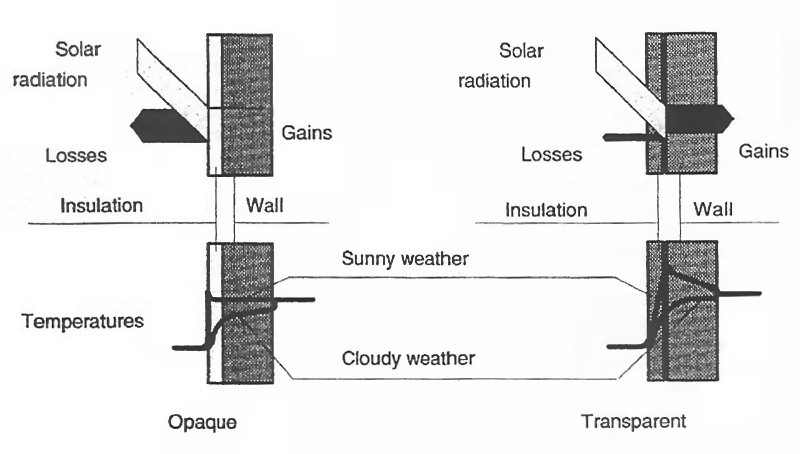
\includegraphics[width=0.9\textwidth, height=0.9\textheight, keepaspectratio=true]{media/image399.png}
\caption{Energy Flows of Opaquely and Transparently Insulated Walls (Wood and Jesch 1993). \protect \label{fig:energy-flows-of-opaquely-and-transparently}}
\end{figure}

While both types of insulation reduce energy losses from the building via conduction through the building surfaces, transparent insulation allows solar radiation to penetrate deeper into the surface construction.~ This increases the construction internal temperature and can result in heat being conducted into the building under the proper weather conditions.~ This can be seen in the lower half of the above figure during a sunny day.~ The temperature plot shows a maximum between the transparent insulation and the rest of the surface construction.~ As a result, the temperature gradient results in heat transfer from this point into the interior space, causing a heating effect on the zone.~ Thus, the advantage of transparent insulation is that, like opaque insulation, it reduces winter heat transfer losses during low or no solar conditions and has the possibility of providing heating during sunny winter days.~ It should be noted that this same effect in summer could be detrimental to the cooling loads of a building since the introduction of solar radiation closer to the space will increase the solar heating within the zone.~ Most systems counteract this with a shading device or with sophisticated transparent insulation systems.

\subsection{Types of Transparent Insulation Materials}\label{types-of-transparent-insulation-materials}

Transparent insulation can be classified into four general categories:

Absorber Parallel Covers

Cavity Structures

Absorber Vertical Covers

Quasi-Homogeneous Structures

Cross-sections of each of these types is shown in the figure below.~ The arrows in these diagrams indicate solar rays and the path these rays trace as they are transmitted through the transparent insulation layer.~ The most advantageous set-up (see absorber-parallel below) would send most of the rays downward towards the interior of the building while minimizing the rays that are reflected back to the exterior environment.

\begin{figure}[hbtp] % fig 27
\centering
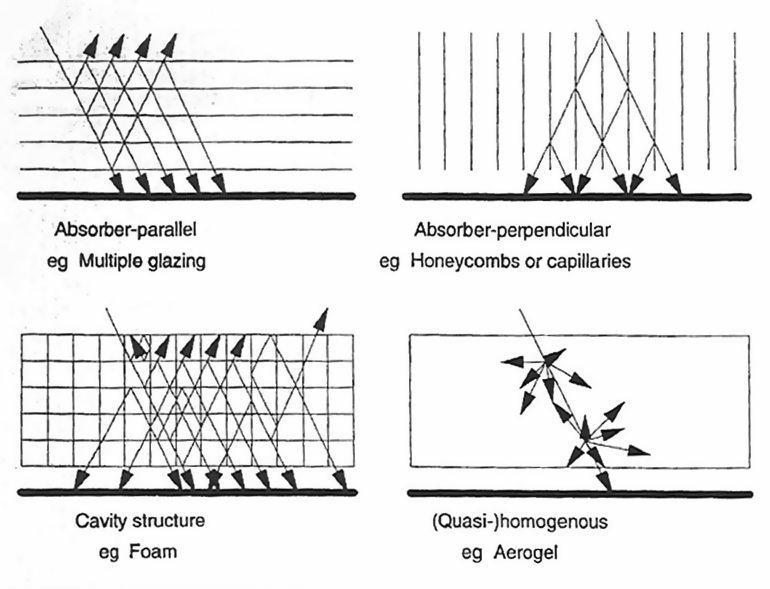
\includegraphics[width=0.9\textwidth, height=0.9\textheight, keepaspectratio=true]{media/image400.png}
\caption{Geometrical Categories of Classification for Transparent Insulation Material (Wood and Jesch 1993). \protect \label{fig:geometrical-categories-of-classification-for}}
\end{figure}

\subsection{TIM- Basic Mathematical Model}\label{tim--basic-mathematical-model}

\begin{figure}[hbtp] % fig 28
\centering
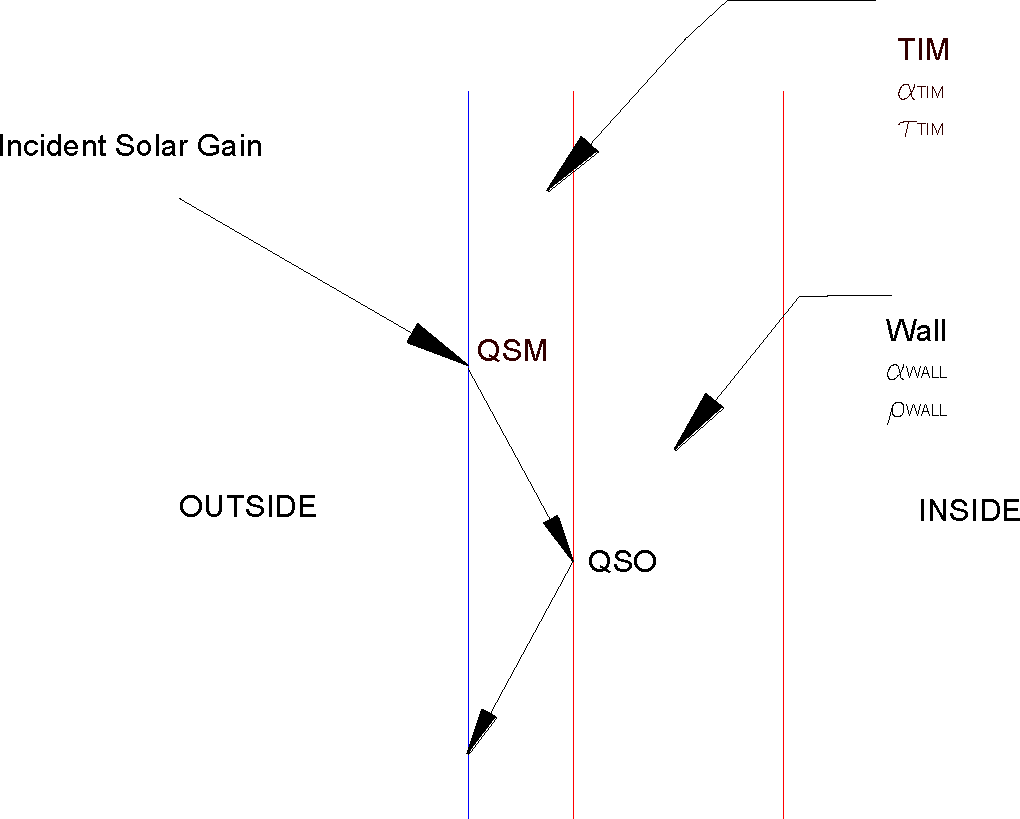
\includegraphics[width=0.9\textwidth, height=0.9\textheight, keepaspectratio=true]{media/image401.png}
\caption{Cross Section of TIM and wall, showing energy flow \protect \label{fig:cross-section-of-tim-and-wall-showing-energy}}
\end{figure}

Mathematical model to calculate amount of energy absorbed at the surface of moveable insulation (TIM) and at the Outside surface of the Wall.

\begin{equation}
QSM = {\alpha_{TIM}}\cdot Incident\;Solar
\label{eq:QSMalphaIncSolar}
\end{equation}

The total solar gain on any exterior surface is a combination of the absorption of direct and diffuse solar radiation given by

\begin{equation}
IncidentSolar = ({I_b}\cdot \cos \theta \cdot \frac{{{S_s}}}{S} + {I_s}\cdot {F_{ss}} + {I_g}\cdot {F_{sg}})
\end{equation}

Where,

$\alpha$ = solar absorptance of the surface

$\theta$ = angle of incidence of the sun's rays

S = area of the surface

S\(_{s}\) = sunlit area of the surface

I\(_{b}\) = intensity of the beam (direct) radiation

I\(_{s}\) = intensity of the sky diffuse radiation

I\(_{g}\) = intensity of the beam (direct) radiation

F\(_{ss}\) = angle factor between the surface and the sky

F\(_{sg}\) = angle factor between the surface and the ground

Now,

\begin{equation}
{\alpha_{wall}} + {\rho_{wall}} = 1
\end{equation}

The model for TIM is simplified in that it assumes that absorption of solar radiation takes place at the inside and outside of the TIM only, not throughout the material.~ In addition, the model assumes that the solar radiation absorbed during the first pass through the TIM affects the outside surface of the TIM while the solar radiation reflected at the outer wall surface that gets absorbed during the back reflection will affect the inside TIM surface (which is also the outside surface of the wall).~ Thus, the heat absorbed at the outside of the TIM is as shown in Equation~\ref{eq:QSMalphaIncSolar}.

The heat absorbed at the inside of the TIM/outside of the wall includes two components.~ The first component is the amount of solar that is transmitted through the TIM and absorbed at the inside of the wall.~ This is characterized by the following equation:

\begin{equation}
First\,pass\,solar\,absorbed\,by\,wall = \left( {{\tau_{TIM}}\cdot Incident\,Solar} \right)\cdot \left( {{\alpha_{wall}}} \right)
\end{equation}

The amount of solar absorbed by the TIM and aggregated at the inside surface of the TIM (outside wall surface) is:

\begin{equation}
Amount\,of\,back\,reflection\,absorbed\,by\,TIM = \left( {{\tau_{TIM}}\cdot Incident\,Solar} \right)\cdot \left( {1 - {\alpha_{wall}}} \right)\cdot {\alpha_{TIM}}
\end{equation}

The heat absorbed at the interface between the wall and the TIM includes both of these components.~ Thus, QSO is equal to:

\begin{equation}
QSO = \left( {{\tau_{TIM}}\cdot Incident\,Solar} \right)\cdot \left\{ {{\alpha_{wall}} + \left( {1 - {\alpha_{wall}}} \right)\cdot \alpha {}_{TIM}} \right\}
\end{equation}

Substituting the definition for QSM into this equation and rearranging results in:

\begin{equation}
QSO = \left\{ {\frac{{{\tau_{TIM}}\cdot QSM}}{{{\alpha_{TIM}}}}} \right\}\cdot \left\{ {{\alpha_{wall}} + \left( {1 - {\alpha_{wall}}} \right)\cdot {\alpha_{TIM}}} \right\}
\end{equation}

\begin{equation}
QSO = \left( {{\tau_{TIM}}\cdot QSM} \right)\cdot \left\{ {\left( {\frac{{{\alpha_{wall}}}}{{{\alpha_{TIM}}}}} \right) + \left( {1 - {\alpha_{wall}}} \right)} \right\}
\end{equation}

Where,

\emph{QSM}~~~~~~~~~~ = Short wave radiant flux absorbed at surface of Movable Insulation

\emph{QSO}~~~~~~~~~~ = Short wave radiant flux absorbed at surface of Wall.

$\alpha$\(_{TIM}\) = Absorptance of TIM

$\tau$\(_{TIM}\) = Transmittance of TIM.

$\alpha$\(_{WALL}\) = Absorptance of Wall.

$\rho$\(_{WALL}\) = Reflectance of Wall surface

Following is the C++ code in the current version of EnergyPlus used in the HeatBalanceSurfaceManager module, to determine the short wave radiation absorbed on outside of movable insulation and the short wave radiation absorbed on outside of opaque surface of the wall.

\begin{lstlisting}
// Calculate absorbed solar on outside if movable exterior insulation in place
HMovInsul = 0.0;
if (Surface(SurfNum).MaterialMovInsulExt > 0) EvalOutsideMovableInsulation(SurfNum, HMovInsul, RoughIndexMovInsul, AbsExt);
if (HMovInsul > 0) { // Movable outside insulation in place
    QRadSWOutMvIns(SurfNum) = QRadSWOutAbs(SurfNum) * AbsExt / Material(Construct(ConstrNum).LayerPoint(1)).AbsorpSolar;
    QRadSWOutAbs(SurfNum) = Material(Surface(SurfNum).MaterialMovInsulExt).Trans * QRadSWOutMvIns(SurfNum) *
                            ((Material(Construct(ConstrNum).LayerPoint(1)).AbsorpSolar / AbsExt) +
                            (1 - Material(Construct(ConstrNum).LayerPoint(1)).AbsorpSolar));
    SWOutAbsTotalReport(SurfNum) = QRadSWOutAbs(SurfNum) * Surface(SurfNum).Area;
    SWOutAbsEnergyReport(SurfNum) = SWOutAbsTotalReport(SurfNum) * TimeStepZoneSec;
}
\end{lstlisting}

\subsection{Sample Test Run Cases: -- Comparison}\label{sample-test-run-cases-comparison}

A series of test cases were run in EnergyPlus to test the TIM model.~ The building was a very simple box with walls facing north, south, east, and west, all of which are exterior walls.~ Transparent Insulation Material has been applied to the south wall (except as noted in the table below).~ The program was run for this fictional 1 zone building located in Chanute AFB IL, for two design days, (21\(^{st}\) June and 21\(^{st}\) January).~ The main purpose of these runs was to verify that the transparent insulation model was predicting results that were reasonable using a simple test case.~ The winter design day was also modified in some runs to have a clearness of 1.0 so that the effect that solar radiation during winter-time conditions could be studied.

The Transparent Insulation material is conceived by applying a SurfaceControl:MoveableInsulation on the exterior.~ In the test cases, the TIM had the following thermal properties:

~~~ 0.05, ! Thickness \{m\}

~~~ 0.90,~ ! Solar transmittance at normal incidence

~~~ 0.031,~ ! Solar reflectance at normal incidence: front side

~~~ 0.031,~ ! Solar reflectance at normal incidence: back side

~~~ 0.90,~ ! Visible transmittance at normal incidence

~~~ 0.05,~ ! Visible reflectance at normal incidence: front side

~~~ 0.05,~ ! Visible reflectance at normal incidence: back side

~~~ 0.0,~~ ! IR transmittance at normal incidence

~~~ 0.84,~ ! IR emissivity: front side

~~~ 0.84,~ ! IR emissivity: back side

~~~ 0.04;~~ ! Conductivity \{W/m-K\}

The Wall Construction is defined as an EXTWALL80 composed of 1'' Stucco, 4'' Common Brick and ¾'' Plaster or Gypboard.

The following two tables shows data for two series of runs.~ The first ``summer table'' illustrates the execution of a summer design day.~ The second ``winter table'' shows winter conditions with clearness = 0 (the typical default for a winter design day) and clearness = 1 (to illustrate solar radiation with other winter conditions).~ Test cases included no movable insulation, moveable opaque insulation, and TIM on the exterior (south wall unless otherwise noted).~ Savings reported are heating and cooling loads for the design days only.~ The results showed that the TIM model was performing reasonably well and was producing results that were within expectations.

% table 14
{\scriptsize
\begin{longtable}[c]{p{2.5in}p{0.75in}p{0.75in}p{0.75in}p{0.75in}}
\caption{TIM with Summer Conditions \label{table:tim-with-summer-conditions-000}} \tabularnewline
\toprule 
EXTWALL80 Construction & Conductivity & Thickness & Sensible Cooling Energy & Energy Saved \tabularnewline
~ & [W/m-K] & [m] & [J] & [J] \tabularnewline
\midrule
\endfirsthead

\caption[]{TIM with Summer Conditions} \tabularnewline
\toprule
EXTWALL80 Construction & Conductivity & Thickness & Sensible Cooling Energy & Energy Saved \tabularnewline
~ & [W/m-K] & [m] & [J] & [J] \tabularnewline
\midrule
\endhead

Normal case Without any Insulation & 0.000 & 0.000 & 3.37E+08 & 0.00E+00 \tabularnewline
With Dense Insulation Present & 0.040 & 0.025 & 3.17E+08 & 2.05E+07 \tabularnewline
With Dense Insulation Present & 0.040 & 0.050 & 3.09E+08 & 2.84E+07 \tabularnewline
With Dense Insulation Present & 0.040 & 0.100 & 3.02E+08 & 3.53E+07 \tabularnewline
With TIM Present & 0.040 & 0.025 & 4.27E+08 & -9.01E+07 \tabularnewline
With TIM Present & 0.040 & 0.050 & 4.63E+08 & -1.26E+08 \tabularnewline
With TIM Present & 0.040 & 0.100 & 4.89E+08 & -1.52E+08 \tabularnewline
With TIM Present R value = (0.05m,0.04W/m-K) & 0.035 & 0.044 & 4.63E+08 & -1.26E+08 \tabularnewline
With TIM Present (EAST WALL) & 0.040 & 0.050 & 5.49E+08 & -2.12E+08 \tabularnewline
With TIM Present (NORTH WALL) & 0.040 & 0.050 & 3.63E+08 & -2.57E+07 \tabularnewline
With TIM Present (WEST WALL) & 0.040 & 0.050 & 5.64E+08 & -2.27E+08 \tabularnewline
\bottomrule
\end{longtable}}

% table 15
{\scriptsize
\begin{longtable}[c]{p{1.0in}p{0.75in}p{0.75in}p{0.75in}p{0.75in}p{0.75in}p{0.75in}}
\caption{TIM with Winter Conditions \label{table:tim-with-winter-conditions-000}} \tabularnewline
\toprule 
EXTWALL80 Construction & Conductivity & Thickness & Sensible Heating Energy & Energy Saved Winter Clearness = 0 & Sensible Heating Energy & Energy Saved Winter Clearness = 1 \tabularnewline
~ & [W/m-K] & [m] & [J] & [J] & [J] & [J] \tabularnewline
\midrule
\endfirsthead

\caption[]{TIM with Winter Conditions} \tabularnewline
\toprule 
EXTWALL80 Construction & Conductivity & Thickness & Sensible Heating Energy & Energy Saved Winter Clearness = 0 & Sensible Heating Energy & Energy Saved Winter Clearness = 1 \tabularnewline
~ & [W/m-K] & [m] & [J] & [J] & [J] & [J] \tabularnewline
\midrule
\endhead

Normal case Without any Insulation & 0.000 & 0.000 & 1.47E+09 & 0.00E+00 & 1.05E+09 & 0.00E+00 \tabularnewline
With Dense Insulation Present & 0.040 & 0.025 & 1.30E+09 & 1.70E+08 & 9.76E+08 & 7.40E+07 \tabularnewline
With Dense Insulation Present & 0.040 & 0.050 & 1.26E+09 & 2.10E+08 & 9.73E+08 & 7.70E+07 \tabularnewline
With Dense Insulation Present & 0.040 & 0.100 & 1.22E+09 & 2.50E+08 & 9.74E+08 & 7.60E+07 \tabularnewline
With TIM Present & 0.040 & 0.025 & 1.30E+09 & 1.70E+08 & 5.66E+08 & 4.84E+08 \tabularnewline
With TIM Present & 0.040 & 0.050 & 1.26E+09 & 2.10E+08 & 4.41E+08 & 6.09E+08 \tabularnewline
With TIM Present & 0.040 & 0.100 & 1.22E+09 & 2.50E+08 & 3.57E+08 & 6.93E+08 \tabularnewline
With TIM Present R value = (0.05m,0.04W/m-K) & 0.035 & 0.044 & 1.26E+09 & 2.10E+08 & 4.40E+08 & 6.10E+08 \tabularnewline
With TIM Present (EAST WALL) & 0.040 & 0.050 & 1.26E+09 & 2.10E+08 & 7.36E+08 & 3.14E+08 \tabularnewline
With TIM Present (NORTH WALL) & 0.040 & 0.050 & 1.24E+09 & 2.30E+08 & 8.31E+08 & 2.19E+08 \tabularnewline
With TIM Present (WEST WALL) & 0.040 & 0.050 & 1.24E+09 & 2.30E+08 & 7.07E+08 & 3.43E+08 \tabularnewline
\bottomrule
\end{longtable}}

\subsection{References}\label{references-046}

P.O. Braun, A. Goetzberger, J. Schmid, and W.Stahl. Transparent Insulation of Building Facades- Steps from Research to Commercial applications, Fraunhofer Institute for Solar Energy Systems, Oltmannsstrasse 22, D-7800 Freiburg, Germany.

Thermotropic materials and Systems for Overheating Protection.

Robert Hausner. Arbeitsgemeinschaft Erneuerbare energie, Transparent Insulation- Areas of Application, Society for Renewable Energy.

Werner J.Platzer. Transparent Insulation materials: a review, Fraunhofer Institute for Solar Energy Systems, Oltmannsstr. 5, D-79100 Freiburg, Germany.

Volker Wittwer. The use of Transparent Insulation Materials and Optical Switching Layers in Window Systems, Fraunhofer Institute for Solar Energy Systems, Oltmannsstr. 5, D-79100 Freiburg, Germany.

M. Wood and L.F. Jesch. 1993. Transparent insulation technology: a technical note, Ambient Press Limited.

Façade Modules with back-ventilated Transparent Insulation- Research and Development toward Series Application.

Two 0-Energy Houses,

Advanced Building Technologies -- Transparent Insulation Materials ( TIM ).

Transparent Insulation,

G. Verbeeck, H. Hens. Transparent Insulation: an alternative solution for summer discomfort. Die neue Transparenz: Warmedamm-Verbund- system StoTherm Solar.

E.Lindauer, H.Leonhardt. Brauchwasservorerwarmmung mit transparent gedammten Bauteilen ( Hybridsystem ), Fraunhofer- Institut fur Bauphysik.
